\documentclass[a4paper]{article}

\usepackage[english]{babel}
\usepackage[utf8]{inputenc}
\usepackage{amsmath}
\usepackage{graphicx}
\usepackage[colorinlistoftodos]{todonotes}
\usepackage{algorithm}
\usepackage[noend]{algpseudocode}

\title{Numerical Methods in Steady State 1D and 2D Heat Equations}

\author{Yuege Xie (EID:yx4256)}
\date{}
\begin{document}
\maketitle
\tableofcontents

\newpage
\section{Introduction}
\label{sec:introduction}

The steady-state heat equation with a constant coefficient in two dimensions is given by:
$$-k\nabla^2u(x,y) = q(x,y)$$
where k is the thermal conductivity, u is the material temperature, and q is a heat source term.\\\\
In this Documentation, we first list some assumptions that help us to simplify and reformulate the 1D and 2D problems. Second, we derive the 2nd and 4th order finite difference expression using node-based central difference. Third, we transform the PDE into linear systems with certain matrices by flattening. Then, we can use Jacobi and Gauss-Seidel iterative methods to solve PDE numerically by solving linear systems. 

\section{Assumptions}
\begin{itemize}
    \item \textbf{Dirichlet Boundary Condition:} The solution is known on the boundary, i.e.
    $$ u(x)|_{x=a,b} = u_0(x)$$
    $$u(x,y)|_{\partial\Omega} = u_0(x,y)$$
    for 1D and 2D cases, respectively, hence the scheme is node-base.
    \item \textbf{Central Finite Difference Method:} use central finite difference for both 2nd order and 4th order approximations.
    \item \textbf{Special Points in 4th Order:} We use 2nd order for the points just near the known boundary, it does not influence the acurracy for center points.
    \item \textbf{Domain Size:} In 2D case, the domain is rectangular, i.e $\Omega = [a_1,b_1] \times [a_2,b_2]$. Moreover, if $b_1-a_1 = b_2-a_2$, it's square, we consider this case.
    \item \textbf{Mesh Size:} $\Delta x = \Delta y = h$, i.e. using square mesh.
    \item \textbf{Scheme:} The computational scheme is node-based.
    \item \textbf{Smoothness:} u is smooth enough that we can do the Taylor expansion.
\end{itemize}

\section{Steady State Heat Equation Numerical Formulation}
\subsection{Governing Equations}
\subsubsection{1D Case}
Using assumptions above, we can reformulate 1D steady-state heat equation with dirichlet boundary condition into:
$$\nabla^2u(x) = q(x), ~~\forall x\in \Omega = [a,b]$$
$$u(a) = u_0(a), ~~u(b) = u_0(b) $$
where $f(x) = -\frac{1}{k}q(x)$
\subsubsection{2D Case}
Using assumptions above, we can reformulate 2D steady-state heat equation with dirichlet boundary condition into:
$$\nabla^2u(x,y) = f(x,y), ~~(x,y)\in \Omega = [a_1,b_1] \times [a_2,b_2]$$
$$u(x,y)|_{\partial\Omega} = u_0(x,y)$$
where $f(x,y) = -\frac{1}{k}q(x,y)$

\subsection{Generate Grid Points}
For 1D case, assume we have $N+1$ points, and let $h=\Delta x$, then 
    $$x_i = a + i*h, i = 0,1,2,...,N$$
    
\begin{figure}
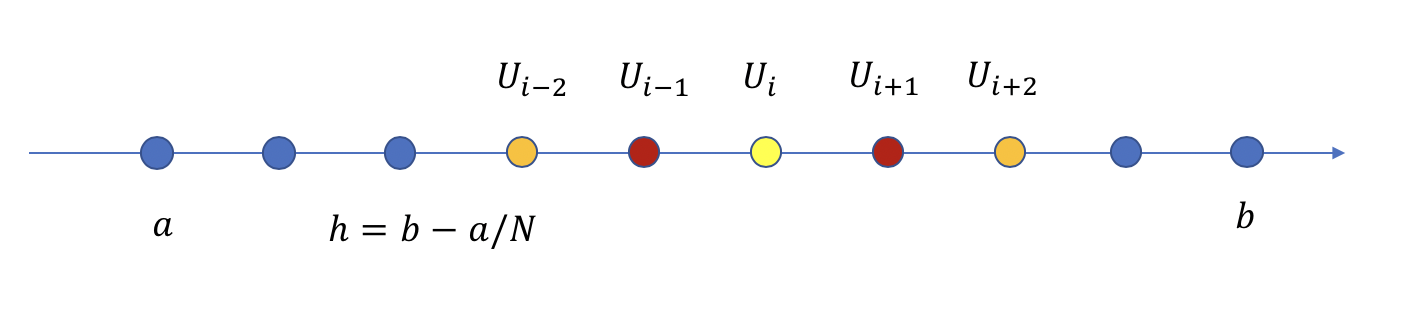
\includegraphics[width=1\textwidth]{1d.png}
\caption{\label{1d}Node-based 1D discretized mesh}
\end{figure}

Let $\Delta x = \Delta y = h = \frac{b_i-a_i}{N_i}$ be the distance between two grid points. Indeed, for rectangular domain, we only have to choose different $N_1$ and $N_2$ to get the same $h$. Then
$$x_i = a_1 + i*h, i = 0,1,2,...,N_1$$
$$y_j = a_2 + j*h, i = 0,1,2,...,N_2$$
We want to get approximations of $U_{ij} = u(x_i,y_j)$ at grid points $(x_i, y_j)$. Since by Dirichlet Boundary Condition, the solution on boundaries are known, we only have $(N_1-1)\times (N_2-1)$ unknowns to solve.

\begin{figure}
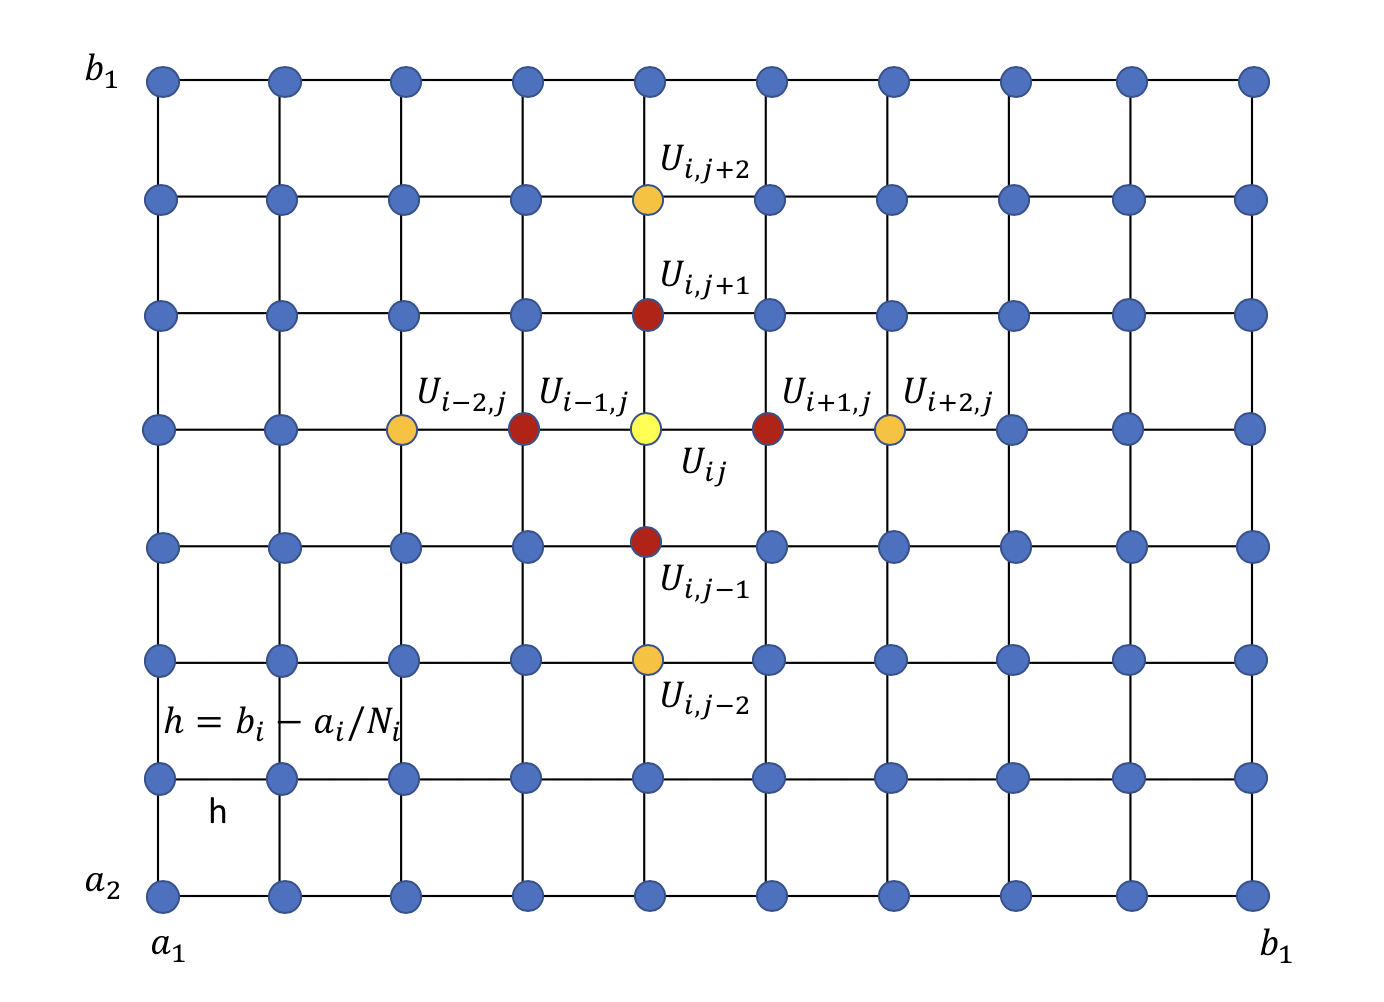
\includegraphics[width=1\textwidth]{2d.png}
\caption{\label{2d}Node-based 2D discretized mesh}
\end{figure}

\subsection{2nd-order Finite Difference Approximation}
\subsubsection{1D Case}
Derived from Taylor expansion of u(x,y), we have
\begin{equation}
    \begin{split}
    \nabla^2u(x_i) = & \frac{u(x_{i-1}) - 2u(x_i) + u(x_{i+1})}{h^2} -\frac{2h^2}{4!}\frac{d^4 u}{d x_i^4} + O(h^4)\\ 
    = & \frac{U_{i-1} - 2U_{i} + U_{i+1} }{h^2} + T_{i}
    \end{split}
\end{equation}

where the local truncation error $T_{i} = -\frac{2h^2}{4!}\frac{d^4 u}{d x_i^4} + O(h^4)$ and we have $\lim_{h\rightarrow 0} T_{i} = 0, \forall i,j$, we can get the following equation:

\begin{equation}
    U_{i-1} - 2U_{i} + U_{i+1}   = h^2 f_{i}
\end{equation}
where $f_i = f(x_i)$,  $i = 1,2,...,N-1$.

\subsubsection{2D Case}
Derived from Taylor expansion of u(x,y), we have

\begin{equation}
    \begin{split}
    \nabla^2u(x_i, y_j) = & \frac{u(x_{i-1},y_j) - 2u(x_i,y_j) + u(x_{i+1},y_j)}{h^2} + \frac{u(x_i,y_{j-1}) - 2u(x_i,y_j) + u(x_i,y_{j+1})}{h^2} \\
    & -\frac{2h^2}{4!}(\frac{\partial^4 u}{\partial x_i^4} + \frac{\partial^4 u}{\partial y_j^4}) + O(h^4)\\ 
    = & \frac{U_{i-1,j} + U_{i+1,j} + U_{i,j-1} + U_{i,j+1} - 4U_{ij} }{h^2} + T_{ij}
    \end{split}
\end{equation}

where the local truncation error $T_{ij} = -\frac{2h^2}{4!}(\frac{\partial^4 u}{\partial x_i^4} + \frac{\partial^4 u}{\partial y_j^4}) + O(h^4)$ and we have $\lim_{h\rightarrow 0} T_{ij} = 0, \forall i,j$, we can get the following equation:

\begin{equation}
    U_{i,j-1} + U_{i-1,j} - 4U_{ij} + U_{i+1,j} + U_{i,j+1}   = h^2 f_{ij}
\end{equation}

where $ i = 1,2,...,N_1-1, j = 1,2,...,N_2-1$ and $f_{ij} = f(x_i,y_j)$

\subsection{4th-order Finite Difference Approximation}

\subsubsection{1D Case}
\begin{equation}
    \nabla^2 u(x_i) = \frac{-U_{i-2,j} + 16U_{i-1,j} - 30U_{ij} + 16 U_{i+1,j} - U_{i+2,j}}{12h^2} -\frac{8h^4}{6!}\frac{d^6 u}{d x_i^6}  + O(h^6)
\end{equation}

where $\lim_{h\rightarrow 0} -\frac{8h^4}{6!}\frac{d^6 u}{d x_i^6}  + O(h^6) = 0, \forall i$. Then we get:
\begin{equation}
     -\frac{1}{12}U_{i-2} + \frac{4}{3}U_{i-1} - \frac{5}{2}U_{i} + \frac{4}{3}U_{i+1} - \frac{1}{12}U_{i+2} = h^2 f_{i}
\end{equation}

where $ i = 2,...,N-2$ and $f_{i} = f(x_i)$. We use 2nd order on $i=1, N-1$.

\subsubsection{2D Case}
Similar as above, ignore the high order term of $h$, we have 
\begin{equation}
    \begin{split}
    \nabla^2 u(x_i, y_j) =  & \frac{-U_{i-2,j} + 16U_{i-1,j} - 30U_{ij} + 16 U_{i+1,j} - U_{i+2,j}}{12(\Delta x)^2}\\
    & + \frac{-U_{i,j-2} + 16 U_{i,j-1} - 30 U_{i,j} + 16U_{i,j+1} -U_{i, j+2} }{12(\Delta y)^2}  + T_{ij}
    \end{split}
\end{equation}

where the local truncation error $T_{ij} = -\frac{8h^4}{6!}(\frac{\partial^6 u}{\partial x^6} + \frac{\partial^6 u}{\partial y^6}) + O(h^6) $ $\lim_{h\rightarrow 0} T_{ij} = 0, \forall i,j$ as well, we can get the equations:
\begin{equation}
     -\frac{1}{12}U_{i-2,j} + \frac{4}{3}U_{i-1,j} - 5U_{ij} + \frac{4}{3} U_{i+1,j} - \frac{1}{12}U_{i+2,j} -\frac{1}{12}U_{i,j-2} + \frac{4}{3} U_{i,j-1} + \frac{4}{3}U_{i,j+1} -\frac{1}{12}U_{i, j+2} = h^2 f_{ij}
\end{equation}

where $ i = 2,...,N_1-2, j = 2,...,N_2-$ and $f_{ij} = f(x_i,y_j)$. We use 2nd order on $i=1, N-1$ or $j=1, N-1$.

\subsection{Linear System of Heat Equation and Matrix Form}
\subsubsection{1D Case}
For 1D case, just let $z=[U_0, U_1,...,U_{N-1},U_N]^T$, where $U_0=u_0(a), U_N=u_0(b)$, then we can get the $Az = b$ form, which can be solved by iterative methods. For 2nd order approximation, with Dirichlet boundary conditions known, we have the following form:
$$b_{2nd} = b_{4th} = b = [ U_0, h^2f_1,...,h^2f_{N-1}, U_N ]^T$$

\[
A_{2nd}^{1D}
=
\begin{bmatrix}
    
    1  &  &   & & & \\
    1  & -2 & 1  &   &  &\\
       & 1  & -2 & 1  &  & \\
     & & \ddots & \ddots & \ddots & & \\
     & & & 1 & -2  & 1&\\
     & & &  &  & 1 \\
\end{bmatrix}
\]
\#nonzeros of interior: 3, except first and last is 2.  

For 4th order approximation, 
\[
A_{4th}^{1D}
=
\begin{bmatrix}
    
    1  &  &   & & & &\\
    1  & -2 & 1  &   &  & &\\
     -\frac{1}{12}  & \frac{4}{3}  & -\frac{5}{2} & \frac{4}{3}  & - \frac{1}{12} & &&\\
     & \ddots& \ddots & \ddots & \ddots & \ddots & \\
    && -\frac{1}{12}  & \frac{4}{3}  & -\frac{5}{2} & \frac{4}{3}  & - \frac{1}{12} \\
     & & & & 1 & -2  & 1\\
     & & & &   &     & 1 \\
\end{bmatrix}
\]
\#nonzeros of interior row: 5, except second and second last is 4, first and first last is 3.

\subsubsection{2D Case}
We want to transform the 2D problem into a linear system $Az=b$ as well and use iterative methods like Jacobi and Gauss-Seidel to solve it.
First, assume $N_1=N_2=N$, flatten $U_{ij}$ into a vector $z$ using rule: 
$$z_{i(N+1)+j} = U_{i,j}, \forall i = 0,1,2,...N, j = 0,1,2,...,N$$
Then we have $z = [U_{00}, U_{01},...,U_{0N},U_{10},...,U_{NN}]^T$.  \\
Second, we use the same rule of adding boundary variables as 1D case to flatten $f$ into $b$:
$$b_{2nd} = b_{4th} = b = [U_{00}, U_{01},..., U_{0,N}, U_{10}, h^2f_{11},...,h^2f_{1,N-1},...,h^2f_{N-1,N-1},U_{N-1,N},...,U_{N,N} ]^T $$
Third, we can get the form of corresponding A:
\[
A_{2nd}^{2D}
=
\begin{bmatrix}
    I &  &   &   &  &\\
    I & B_{2nd} & I  &   &  &\\
     & & \ddots & \ddots & \ddots & & \\
     & & & I& B_{2nd}  & I& \\
     & & &  &  & I  \\
\end{bmatrix}
\]
where $I=I_{N+1\times N+1}$ and $B$ is also $N+1 \times N+1$ matrix.\\
\#nonzeros of interior row: 5, except first and last is 4. 
\[
B_{2nd} = 
\begin{bmatrix}
    1 & -4 & 1  &    &   &   &\\
      &  1 & -4 & 1  &   &   &\\
      &     & \ddots & \ddots & \ddots & & \\
     & & & 1& -4  & 1 & \\
     & & &  & 1 & -4  &1\\
\end{bmatrix}
\]

\begin{figure}
\centering
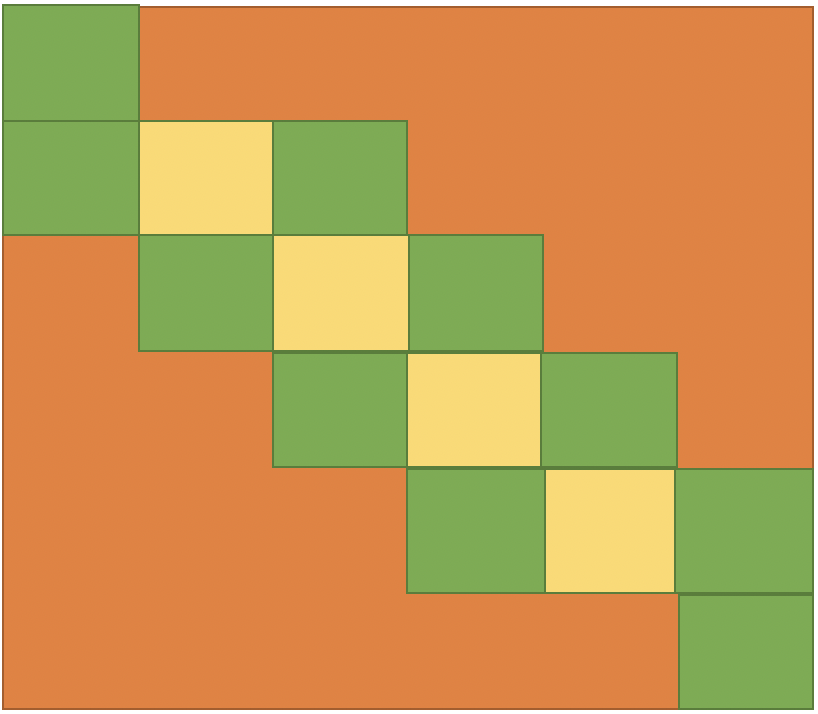
\includegraphics[width=0.4\textwidth]{2nd.png}
\caption{\label{2nd}Structure of 2nd order difference matrix}
\end{figure}

For 4th order approximation, we only use 2nd order approximation on the points with indices $1$ and $N-1$:

\[
A_{4th}^{2D}
=
\begin{bmatrix}
    I &  &   &   &  &\\
    I & C_{4th} & I  &   &  &\\
    -\frac{1}{12}I& \frac{4}{3}I & B_{4th} & \frac{4}{3}I & -\frac{1}{12}I \\
     & &\ddots& \ddots & \ddots & \ddots & \ddots& \\
     &&-\frac{1}{12}I& \frac{4}{3}I & B_{4th} & \frac{4}{3}I & -\frac{1}{12}I \\
     & & & &I& C_{4th}  & I& \\
     & & &  & &  & I  \\
\end{bmatrix}
\]
where $I=I_{N+1\times N+1}$ and $B$ is also $N+1 \times N+1$ matrix.\\
\#nonzeros of interior row: 9, except boundary cases.

\[
B_{4th}
=
\begin{bmatrix}
    1 & -\frac{9}{2} &1\\
    -\frac{1}{12}  & \frac{4}{3}  & -5 & \frac{4}{3}  & - \frac{1}{12} & &&\\
     &-\frac{1}{12}  & \frac{4}{3}  & -5 & \frac{4}{3}  & - \frac{1}{12} & &&\\
     && \ddots& \ddots & \ddots & \ddots & \ddots & \\
    &&& -\frac{1}{12}  & \frac{4}{3}  & -5 & \frac{4}{3}  & - \frac{1}{12} \\
    &&&& -\frac{1}{12}  & \frac{4}{3}  & -5 & \frac{4}{3}  & - \frac{1}{12} \\
     &&&& &&1 & -\frac{9}{2} &1\\
\end{bmatrix}
\]

\[
C_{4th}
=
\begin{bmatrix}
    1 & -4 &1\\
    -\frac{1}{12}  & \frac{4}{3}  & -\frac{9}{2} & \frac{4}{3}  & - \frac{1}{12} & &&\\
     &-\frac{1}{12}  & \frac{4}{3}  & -\frac{9}{2} & \frac{4}{3}  & - \frac{1}{12} & &&\\
     && \ddots& \ddots & \ddots & \ddots & \ddots & \\
    &&& -\frac{1}{12}  & \frac{4}{3}  & -\frac{9}{2} & \frac{4}{3}  & - \frac{1}{12} \\
    &&&& -\frac{1}{12}  & \frac{4}{3}  & -\frac{9}{2} & \frac{4}{3}  & - \frac{1}{12} \\
    &&&& &&1 & -4 &1\\
\end{bmatrix}
\] 
\begin{figure}
\centering
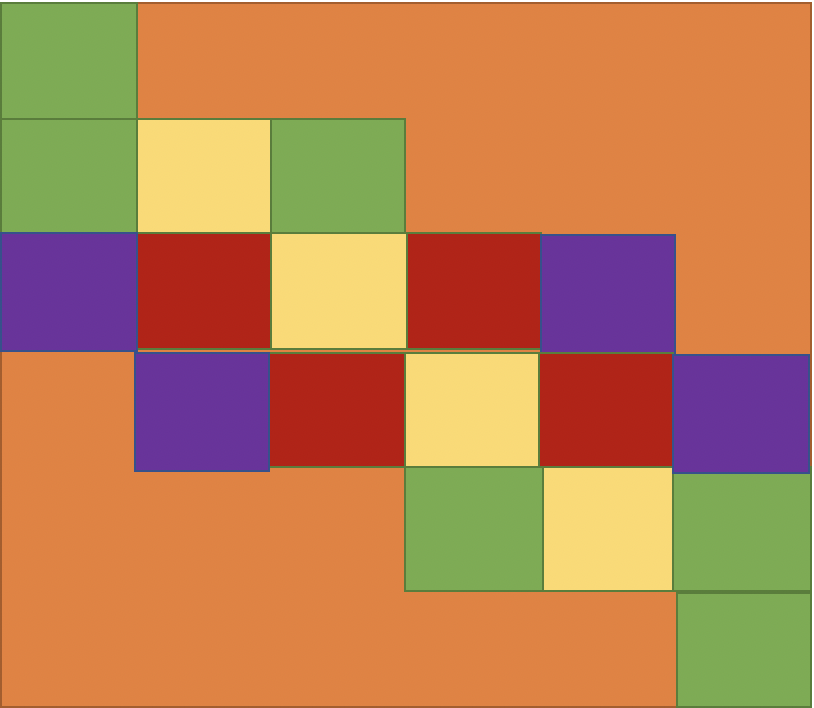
\includegraphics[width=0.4\textwidth]{4th.png}
\caption{\label{4th}Structure of 4th order difference matrix}
\end{figure}

\subsection{Iterative Methods to Solve Linear Systems}
\subsubsection{Jacobi Iterative Method}
Given an initial guess $\mathbf{z}^0$, then the rule of Jacobi iterative method is 
$$z_i^{k+1} = \frac{1}{a_{ii}}(b_i-\sum_{j=1,j\neq i}^n a_{ij}z_j^k)$$

\subsubsection{Gauss-Seidel Iterative Method}
Given an initial guess $\mathbf{z}^0$, then the rule of Gauss-Seidel iterative method is 
$$z_i^{k+1} = \frac{1}{a_{ii}}(b_i-\sum_{j=1}^{i-1} a_{ij}z_j^{k+1}-\sum_{j=i+1}^{n} a_{ij}z_j^{k})$$

\section{Algorithm}
\begin{algorithm}
\caption{Numerical Methods to Solve Steady State Heat Equations}
    \begin{algorithmic}
    \State \textbf{Input:} tolerance $\epsilon >0$, max\_iter, iter\_method, dim, fd\_method, domain, $N, q(x,y)$, boundary $u_0(x,y)$ or $u_0(a), u_0(b)$.
    \State \textbf{Output:} $u(x_i,y_j), i = 1,2,...,N-1, j = 1,2,...,N-1$ 
    \State \textbf{Initialize:} k = 0, error = 1000, $f(x_i,y_j) = -\frac{1}{k}q(x_i,y_j)$
        \If{dim == 1}
            $$z=[U_0, U_1,...,U_{N-1},U_N]^T$$
            $$b = [ U_0, h^2f_1,...,h^2f_{N-1}, U_N ]^T$$
            
            \If{fd\_method == 2nd}
            $$A = A_{2nd}^{1D}$$
            \Else
            $$A = A_{4th}^{1D}$$
            \EndIf
        \EndIf
        
        \If{dim == 2} 
             $$z = [U_{00}, U_{01},...,U_{0N},U_{10},...,U_{NN}]^T$$
             $$b = [U_{00}, U_{01},..., U_{0,N}, U_{10}, h^2f_{11},...,h^2f_{1,N-1},...,h^2f_{N-1,N-1},U_{N-1,N},...,U_{N,N} ]^T $$
            \If{fd\_method == 2nd}
            $$A = A_{2nd}^{2D}$$
            \Else
            $$A = A_{4th}^{2D}$$
            \EndIf
        \EndIf
    
        \While { error $> \epsilon$ and k $<=$ max\_iter }
        
        
        \If {iter\_method == Jacobi}
        \For {$i=0,1,2,..,N$}
        sum = 0
        \For {$j=0,1,2,...,N$}
        \If{$j\neq i$}
        $sum = sum+a_{ij}z_j^k$
        \EndIf
        \EndFor
        $z_i^{k+1} = \frac{1}{a_{ii}}(b_i-sum)$
        \EndFor
        \EndIf
        
        
        \If {iter\_method == Gauss\_Seidel}
        \For {$i=0,1,2,..,N$}
        sum = 0
        \For {$j=0,1,2,...,i-1$}
        $sum = sum+a_{ij}z_j^{k+1}$
        \EndFor
        \For {$j=i+1,i+2,...,N$}
        $sum = sum+a_{ij}z_j^k$
        \EndFor
        $z_i^{k+1} = \frac{1}{a_{ii}}(b_i-sum)$
        \EndFor
        
        \EndIf
         
        \State error = $\|b-Az\|_2$
        \State $k \leftarrow k+1$

        \EndWhile
    \Return $z^k$
    \end{algorithmic}
\end{algorithm}

\section{Memory Estimate}
Memory that we need includes the following things:
\begin{itemize}
    \item \textbf{Iteration Variables:} matrix A, vector b, vector z, $k$, error
    \item \textbf{Inputs:} tolerance $\epsilon$, max\_iter, iter\_method, dim, fd\_method, domain, $N$.
\end{itemize}

\begin{enumerate}
    \item For matrix A, because it has special diagonal structures, we can use sliding method to do the iteration instead of so we only need to store constant number of it, which is at most 9 non-zeros. We can estimate 10 doubles for A.
    \item For inputs and iteration variables $k$, error, we only need 1 double to store them, they are 9 in total, and we can estimate 10 doubles for them.
    \item For x and b, we need $N+1$ for 1D case and $(N+1)^2$ for 2D case, respectively.
\end{enumerate}

The difference between Jacobi and Gauss-Seidel iterations is that we update the variable in Gauss-Seidel iteration in the loop, so we only need one x to store it. But for Jacobi, we update them until we get all the new values for a new iteration, so we need at least two x to store them.

And we need 8B to store a double, then the total memory we need is as follows in Table \ref{table}.

\begin{table}[]
\centering
\begin{tabular}{l|l|lll}
\hline
iter\_method/dim & 1D & 2D \\
\hline
Jacobi& $(3\times (N+1)+ 20)\times 8B$ & $(3\times (N+1)^2+ 20)\times 8B$   \\
Gauss-Seidel & $(2 \times (N+1)+ 20)\times 8B$ & $(2\times (N+1)^2+ 20)\times 8B$  \\
\hline
\end{tabular}
\caption{\label{table}Memory Estimate Summary}
\end{table}

\end{document}